\chapter{Background}
%
% lead sulfide important - study everything about it. Also it's in space. Study radiation damage.
% BGU made a thing. They studied it some. Let's study it some more.
% TGS has been happening at MIT. This is just the next thing we can study it with.
% There's a search for model radiation damage systems.
This work is the result of three separate avenues of progress that happened to converge. They are summarized here and elaborated upon later:
\begin{enumerate}
	\item Recent work to hone chemical bath deposition of PbS culminated in growing thin films of PbS doped with thorium.\label{first_avenue}
	\item Transient grating spectroscopy (TGS) is an emerging tool for studying radiation damage, and its suitability for studying thin films, whether semiconductor or otherwise, has become apparent.\label{second_avenue}
	\item Radiation materials scientists are interested in teasing apart the different radiation damage mechanisms and determining the contribution of each to changes in bulk parameters (such as Young's modulus, strength, resistivity, etc.). Thorium doped PbS holds promise as a ``model system'' for studying radiation damage.\label{third_avenue}
\end{enumerate}
The confluence of motives and methods in this work will defy intuition should the reader not take a moment first to understand that it serves these three separate needs simultaneously.

In Templeman et al. 2017, a team at Ben-Gurion University announced successful doping of a lead sulfide thin film with radioactive Th-228, which they hailed as a new ``model system'' for radiation damage studies. Earlier papers from the same team do not hint that radiation damage studies were their ultimate goal. For instance, Templeman et al. 2014 is simply about the effect of pH and the order of reagent addition on the growth of lead selenide \cite{Templeman2014}. At some point, however, the team realized that doping PbS with Th-228 was worthy of pursuit, and several papers clearly build toward this goal. In particular, Biton et al. 2014 explicitly sets out to alloy PbS with the more common and less radioactive Th-232 in preparation for using Th-228 later \cite{Biton2014}.

Semiconductors and their responses to radiation damage are worthy of study, but an obvious and widely available choice like bulk silicon requires a beam line or reactor. For Si, \emph{in situ} or self-irradiation studies do not make for an easier alternative. One cannot simply add radioactive material to a silicon crystal and isolate the effect of the radiation from the effect of a foreign species in the crystal lattice.\footnote{Hence the pains taken by the BGU team to determine whether thorium could indeed be alloyed with PbS without disturbing the lattice. They confirmed thorium was distributed throughout, and the absence of any phases other than rock salt PbS. \cite{Templeman2017}} Furthermore, radioactive materials are in shorter and more controlled supply than semiconductor materials, so the choice of radioactive material actually comes first, and the choice of semiconductor follows.

Thorium 232 is widely available, and thorium 228 happens to be one of its more active daughters, so it is a perfectly reasonable choice of radioisotope. It also makes sense in light of the BGU team's previous experience with growth of lead chalcogenide thin films: lead is the closest stable nucleus to thorium (or any of the naturally occurring radioisotopes), and lead is the final stable daughter of the thorium decay chain. In summary, though Th-228 is not the only possible choice of radioisotope, and PbS is not the archetypical semiconductor, they make sense together.

Once this line of reasoning is accepted, chemical bath deposition (CBD) as a technique and thin films as a product---rather than bulk materials---are simply consequences. Given current techniques of deposition and alloying, growing crystalline or polycrystalline PbS with a controlled quantity of Th-228 uniformly dispersed throughout necessitates CBD. And CBD, while in theory capable of producing thicker-than-thin films, is essentially only used for making thin films, especially in the case of PbS. In summary, dispersing Th-228 in the PbS crystal requires CBD, and CBD produces thin films.

The discussion so far amounts to an understanding of the present work in the context of the first avenue of progress mentioned above (\ref{first_avenue}). For the third (\ref{third_avenue}), the exciting component is the band gap and quantum confinement features of lead sulfide. The promise of semiconductors doped with radioactive materials as ``model systems'' for studying radiation damage stems from the hope that certain types of radiation damage will have different, distinguishable effects on band gap, grain size, and grain boundary \cite{Templeman2017}; all packaged in a sample that produces very little biologically damaging radiation and requires no handling restrictions \cite{Templeman2017}. By analyzing these material parameters over time, it is hoped that the accumulation and evolution of each type of damage can be better understood. For instance, we know that dislocation loops take more time and damage to appear, but what if a change in band gap indicated their quantity exactly at any time?

The second avenue of progress (\ref{second_avenue}), dictates the quantities measured in this work. We have established the justification for lead sulfide, for doping with Th-228, for using CBD, and for producing thin-films. But these two lines of thinking would suggest measuring resistivity, band gap, grain size, or energy barrier at grain boundary. Instead, in this work we opt to measure thermal diffusivity and surface acoustic wave (SAW) speed (a proxy for elasticity). Resistivity has already been characterized in this sample by Templeman et al. 2017 \cite{Templeman2017}, so it makes sense to study a different quantity. And though band gap might be a more intuitive choice, TGS makes it exceedingly easy to study thermal diffusivity and SAW speed. These quantities are not beside the point because they too convey important information about energy levels in the band gap affecting charge carrier mobility and the presence of defects to scatter phonons.

% If just interested in thermal diffusivity, then why report about elasticity? Because TGS
% If just interested in TGS, then why study BGU? Because they made it.
% If just interested in model material, why not measure band gap? Because TGS
% if just interested in radiation damage in PbS, then why not use bulk? Because this is uniformly damaging.


\section{Semiconductor physics and prediction}
In metals, electrical conductivity and thermal conductivity are seemingly linked; an observation that is formalized in the Wiedemann-Franz relation,
\begin{equation}
\frac{\kappa}{\sigma} = LT.
\end{equation}
Although not exactly true, this relationship holds because electrical and thermal conductivity in metals are both dominated by the same parameter: the high mobility of charge carriers, i.e. electrons \cite{Lavasani2018}. The effect of radiation damage on electrical and thermal conductivity can thus be understood in terms of its effect on electron mobility. The story for semiconductors becomes more complicated.

It is still true that electrical conductivity depends on the concentration of charge carriers and the mobility of charge carriers:
\begin{equation}
\sigma = en_p\mu_h + en_e\mu_e.
\end{equation}
But in semiconductors, density of charge carriers is no different than a metal or any other material of similar atomic number, and instead mobility of charge carriers becomes the limiting factor.

Concerning thermal conductivity, there are two mechanisms: charge carriers and phonons. Phonons, the quasi-particles that represent the solid's normal vibrational modes, are a means of thermal conductivity in metals as well, but their contribution is small compared to that of charge carriers. In semiconductors, because the charge carrier mobility is low, the phonon contribution matters.

So, in semiconductors, electrical conductivity is governed by charge carrier mobility, but thermal conductivity is governed by charge carrier mobility and phonon transport. This is why something like the Wiedemann-Franz relation does not exist for semiconductors, and is why we cannot expect radiation damage to have the same effect on thermal conductivity as it does on electrical conductivity.
% semiconductor: thermal diffusivity depends on charge carriers and also phonon transport. Metals have this too, it's just that phonons barely matter. Anyway, phonons scatter off defects.
% semiconductor: electrical conductivity depends on charge carrier mobility
% 
%[Needs rearranging]

The key defining feature of the semiconductor is the band gap: the region of forbidden electron energy and momentum levels between the material's valence and conduction bands. In order to conduct, an electron must absorb a minimum amount of energy and momentum to jump the gap, leaving behind a positively charged ion: a "hole". The electron remains in the conduction band until it finds a hole to recombine with; relaxing back to the valence band by releasing a photon.

We therefore expect radiation damage to affect charge carrier mobility through introducing new energy levels into the band gap, thus reducing the energy necessary for conduction. We expect radiation damage to affect phonon transport through creation of defects, leading to more phonon scattering. For thermal diffusivity, it is not clear which of these hypothesized mechanisms should dominate, since more charge carrier mobility would tend to increase thermal diffusivity and more phonon scattering should reduce thermal diffusivity. Since phonon transport dominates without radiation damage, we expect that reducing this quantity will dominate, and thermal diffusivity will be reduced by damage. For SAW speed, only phonon transport can have an effect, since SAWs can be thought of mathematically as low frequency phonons. Therefore, radiation damage ought to decrease SAW speed. This also satisfies intuition, since crystals in general have higher SAW speeds than amorphous materials.

%[More to say]

%Any semiconductor that starts neutral thus contains an equal number of electrons and holes at all times.

%[Orphan paragraph:]
%The direct band gap of lead sulfide means that, unlike better known semiconductors like silicon, the closest approach between the valence band and the conduction band, energy-wise, does not require any momentum. This makes it conceptually simpler than many semiconductors, but momentum still plays a roll in lead sulfide's thermal properties.
%
%[Orphan paragraph:]
%Usually, electrons in semiconductors acquire the momentum they need to conduct from the solid's vibrational normal modes, called phonons. Since any arbitrary set of motions of a solid's constituent atoms can be decomposed into a sum of normal modes, all kinetic energy within a solid, from acoustic to thermal, can be thought of as a population of phonons. The lower frequencies are associated with acoustics, and the higher ones with thermal properties. 


%\emph{[Insert figure with band structure (E vs. k) for Si and PbS)]}

%Semiconductor optical, electrical, and thermal behavior always comes down to consideration of mobility of charge carriers, phonon population, and band gap. 

\section{Transient Grating Spectroscopy - TGS}
Transient Grating Spectroscopy (TGS) was developed incrementally, but begins with Cachier's work at the Laboratoire d'Ultrasons in Paris in 1970 \cite{Cachier2003}. Lately, TGS crafted according to the specifications of Johnson et al. 2012 \cite{Johnson2012} was set up at MIT under the auspices of the Mesoscale Nuclear Materials Group \cite{Cometto2018}. TGS enables the determination of a sample's material properties by using lasers to excite and measure the propagation of surface acoustic waves (SAWs). It has a host of advantages as a non-destructive, non-contact, rapid assay; but as a surface to mesoscale depth assay, it is especially appropriate for studying thin films and low-penetration radiation damage.

\begin{figure}[thb]
\begin{center}
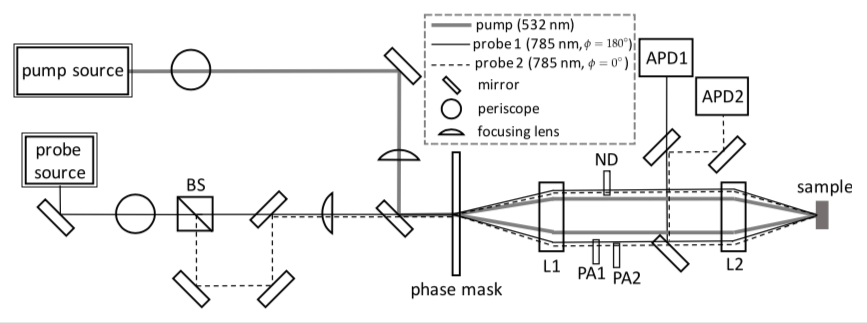
\includegraphics[width=\textwidth]{./images/TGS-DH_setup_Dennet_2017b_1.png}
\caption{Typical TGS setup. L1 and L2 are focusing lenses; ND is a neutral density filter; PA1 and PA2 represent phase adjustments; and APD1 and APD2 are the avalanche photodiodes which collect the reflected probe beam. Image adapted from Dennett and Short 2017 \cite{Dennett2017}.}
\label{TGS_setup}
\end{center}
\end{figure}

Figure \ref{TGS_setup} illustrates a typical TGS setup. Two lasers of the same wavelength $\lambda_{0}$ and phase are aimed at the sample such that the beams overlap and interfere at the sample surface. In this setup, each laser, called a pump beam, mirrors the angle $\theta$ from normal of the other. Both beams are linearly polarized, so where the beams overlap, which we call the footprint, interference will create parallel lines of constructive interference. Where there is constructive interference, the material will experience heating and expansion, uplifting a tiny ripple on the material surface. The lasers are shut off, but the ripples begin to propagate outward and decay as soon as they are created; a process which depends on the material's elasticity and thermal diffusivity. A third laser, called the probe beam, is directed at a fixed location within the footprint, such that the ripples travel beneath it and reflect the probe beam at varying angles. By detecting the reflected beam and its changing angle in avalanche photodiodes, we can deduce the shape and speed of the ripple beneath the probe beam. The resultant signal over time represents the ripples as they travel underneath the probe beam. Refer to Figure \ref{TGS_sample_output}. The oscillations in this curve represent the ripples due the constructive interference of the pump beams; frequency depends on the material's Young's modulus; and time decay depends on the material's thermal diffusivity.

\begin{figure}[thb]
\begin{center}
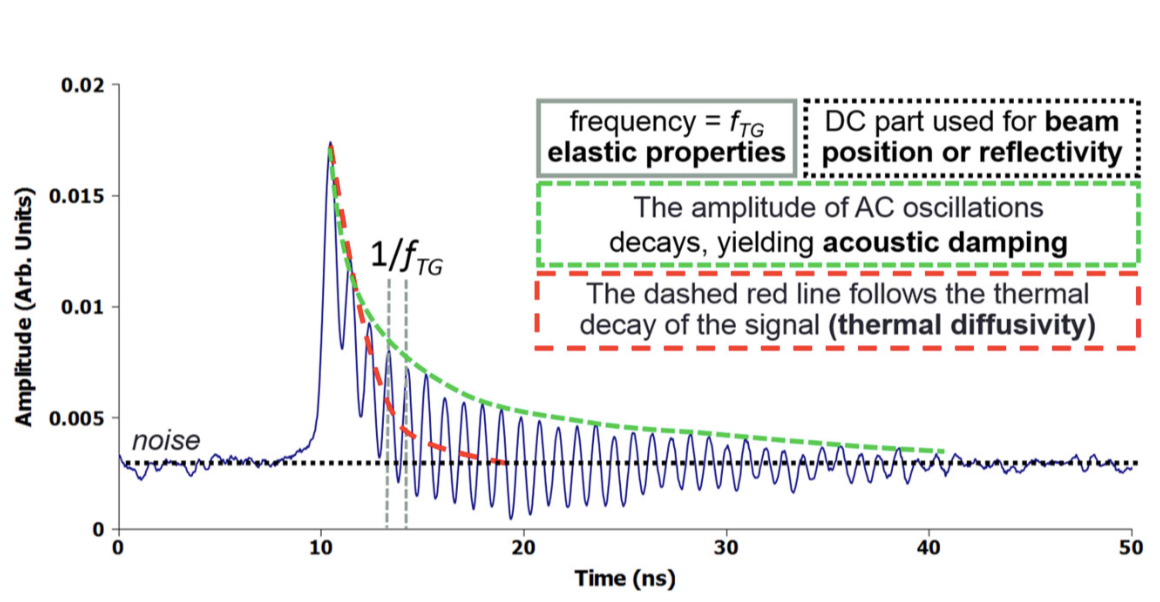
\includegraphics[width=\textwidth]{./images/Sample_TGS_output_2.png}
\caption{Generic TGS output signal plotted with known useful decomposable components called out. Image adapted from Short et al. 2015 \cite{Short2015}.}
\label{TGS_sample_output}
\end{center}
\end{figure}

The ripples continue to the edge of each grain, where they experience some reflection and some transmission to adjacent grains. At the edge of the sample, they reflect. These edge effects can alter the signal picked up by the probe beam, so it is essential that the grain size either be much larger or much smaller than the footprint of the pump lasers. Larger so that reflected waves do not return in time to be recorded; or smaller so that there are enough grains over which to average the grain boundary effect.

If the wavelength of probe beam is $\lambda_0$, then we can expect the wavelength of the ripples of constructive interference to be
$\lambda = \lambda_0 sin(\theta)$, where theta is, again, the angle from normal.

%[Trying to understand how thickness matters. Can a sample be too thin for TGS? Will the GaAs substrate of the PbS(Th) sample have an effect on the results reported from TGS?]

The areas of local heating on the sample surface also penetrate into the material, requiring consideration of the material thickness and desired depth of study. This has an acoustic and thermal component governed by the material speed of sound and the thermal diffusivity, respectively. The acoustic component is therefore roughly immediate and requires that the defects to be studied are within one $\lambda$ of the surface. The thermal component takes longer, and therefore doesn't affect the signal recorded by the probe beam.

In this work, the key consideration is not that the radiation damage is beyond one $\lambda$ from the surface, but rather that the entire thin film is thinner than $\lambda$. The SAW travels parallel to the film-substrate boundary, but the amplitude is such that lead and sulfur atoms will exert pressure on the gallium and arsenic atoms in the substrate. At this boundary, as in all coupled oscillator systems, there is some amount of reflection and transmission of the energy to the substrate. While this affect could be modeled and deconvolved, in this work we assume that since it is present in both the pre-annealing radiation damaged measurements and the post-annealing measurements, it affects all results equally. The thermal diffusivity and SAW speed results should not be expected to match the values of bulk PbS or bulk PbS(Th). Rather, the \emph{percent changes} should match.

\section{Sample preparation}
The thorium doped PbS thin film was prepared by chemical bath deposition (CBD) before the present work began. Templeman et al. 2017 \cite{Templeman2017} describe the process in detail, but it is summarized here for completion. The GaAs (100) substrate was submerged in a chemical bath containing thorium 228. The thorium concentration, temperature, and pH were all precisely varied to control the concentration of thorium incorporated into the PbS rock salt lattice; a method that was confirmed to work by Biton et al. 2014 \cite{Biton2014}. The thorium added to the solution had already aged $\sim$2.5 years since it was created in presumably pure form. Therefore, its daughters were also present in the solution, and Templeman et al. confirmed by gamma and alpha spectroscopy that at least some of the daughters were incorporated into the lattice as well, though they did not attempt to deduce or measure concentrations. The sample properties as reported by Templeman et al. 2017 are collected in Table \ref{sample_properties} and a photo of the sample can be seen in Figure \ref{photo_of_thin_film_sample}.

%\begin{table}[hb]
%\begin{center}
%\begin{tabular}{|l|l|}\hline
%Substrate						&	GaAs (100) \\\hline
%Dimensions					&	1 cm x 1.5 cm \\\hline
%Film thickness					&	$\sim$500 nm \\\hline
%Grain size						&	$\sim$150 nm \\\hline
%Th 228 concentration			&	0.15 ppm \\\hline
%Total activity*					&	65 Bq \\\hline
%Sample creation date			&	22 Jul 2016\\\hline
%\end{tabular}
%\end{center}
%\label{sample_properties}
%\caption{Sample properties reported by Templeman et al. 2017 \cite{Templeman2017}. * Total activity measured a brief but unknown time after sample preparation.}
%\end{table}


\begin{figure}[tbp]
\begin{floatrow}
\ffigbox{%
  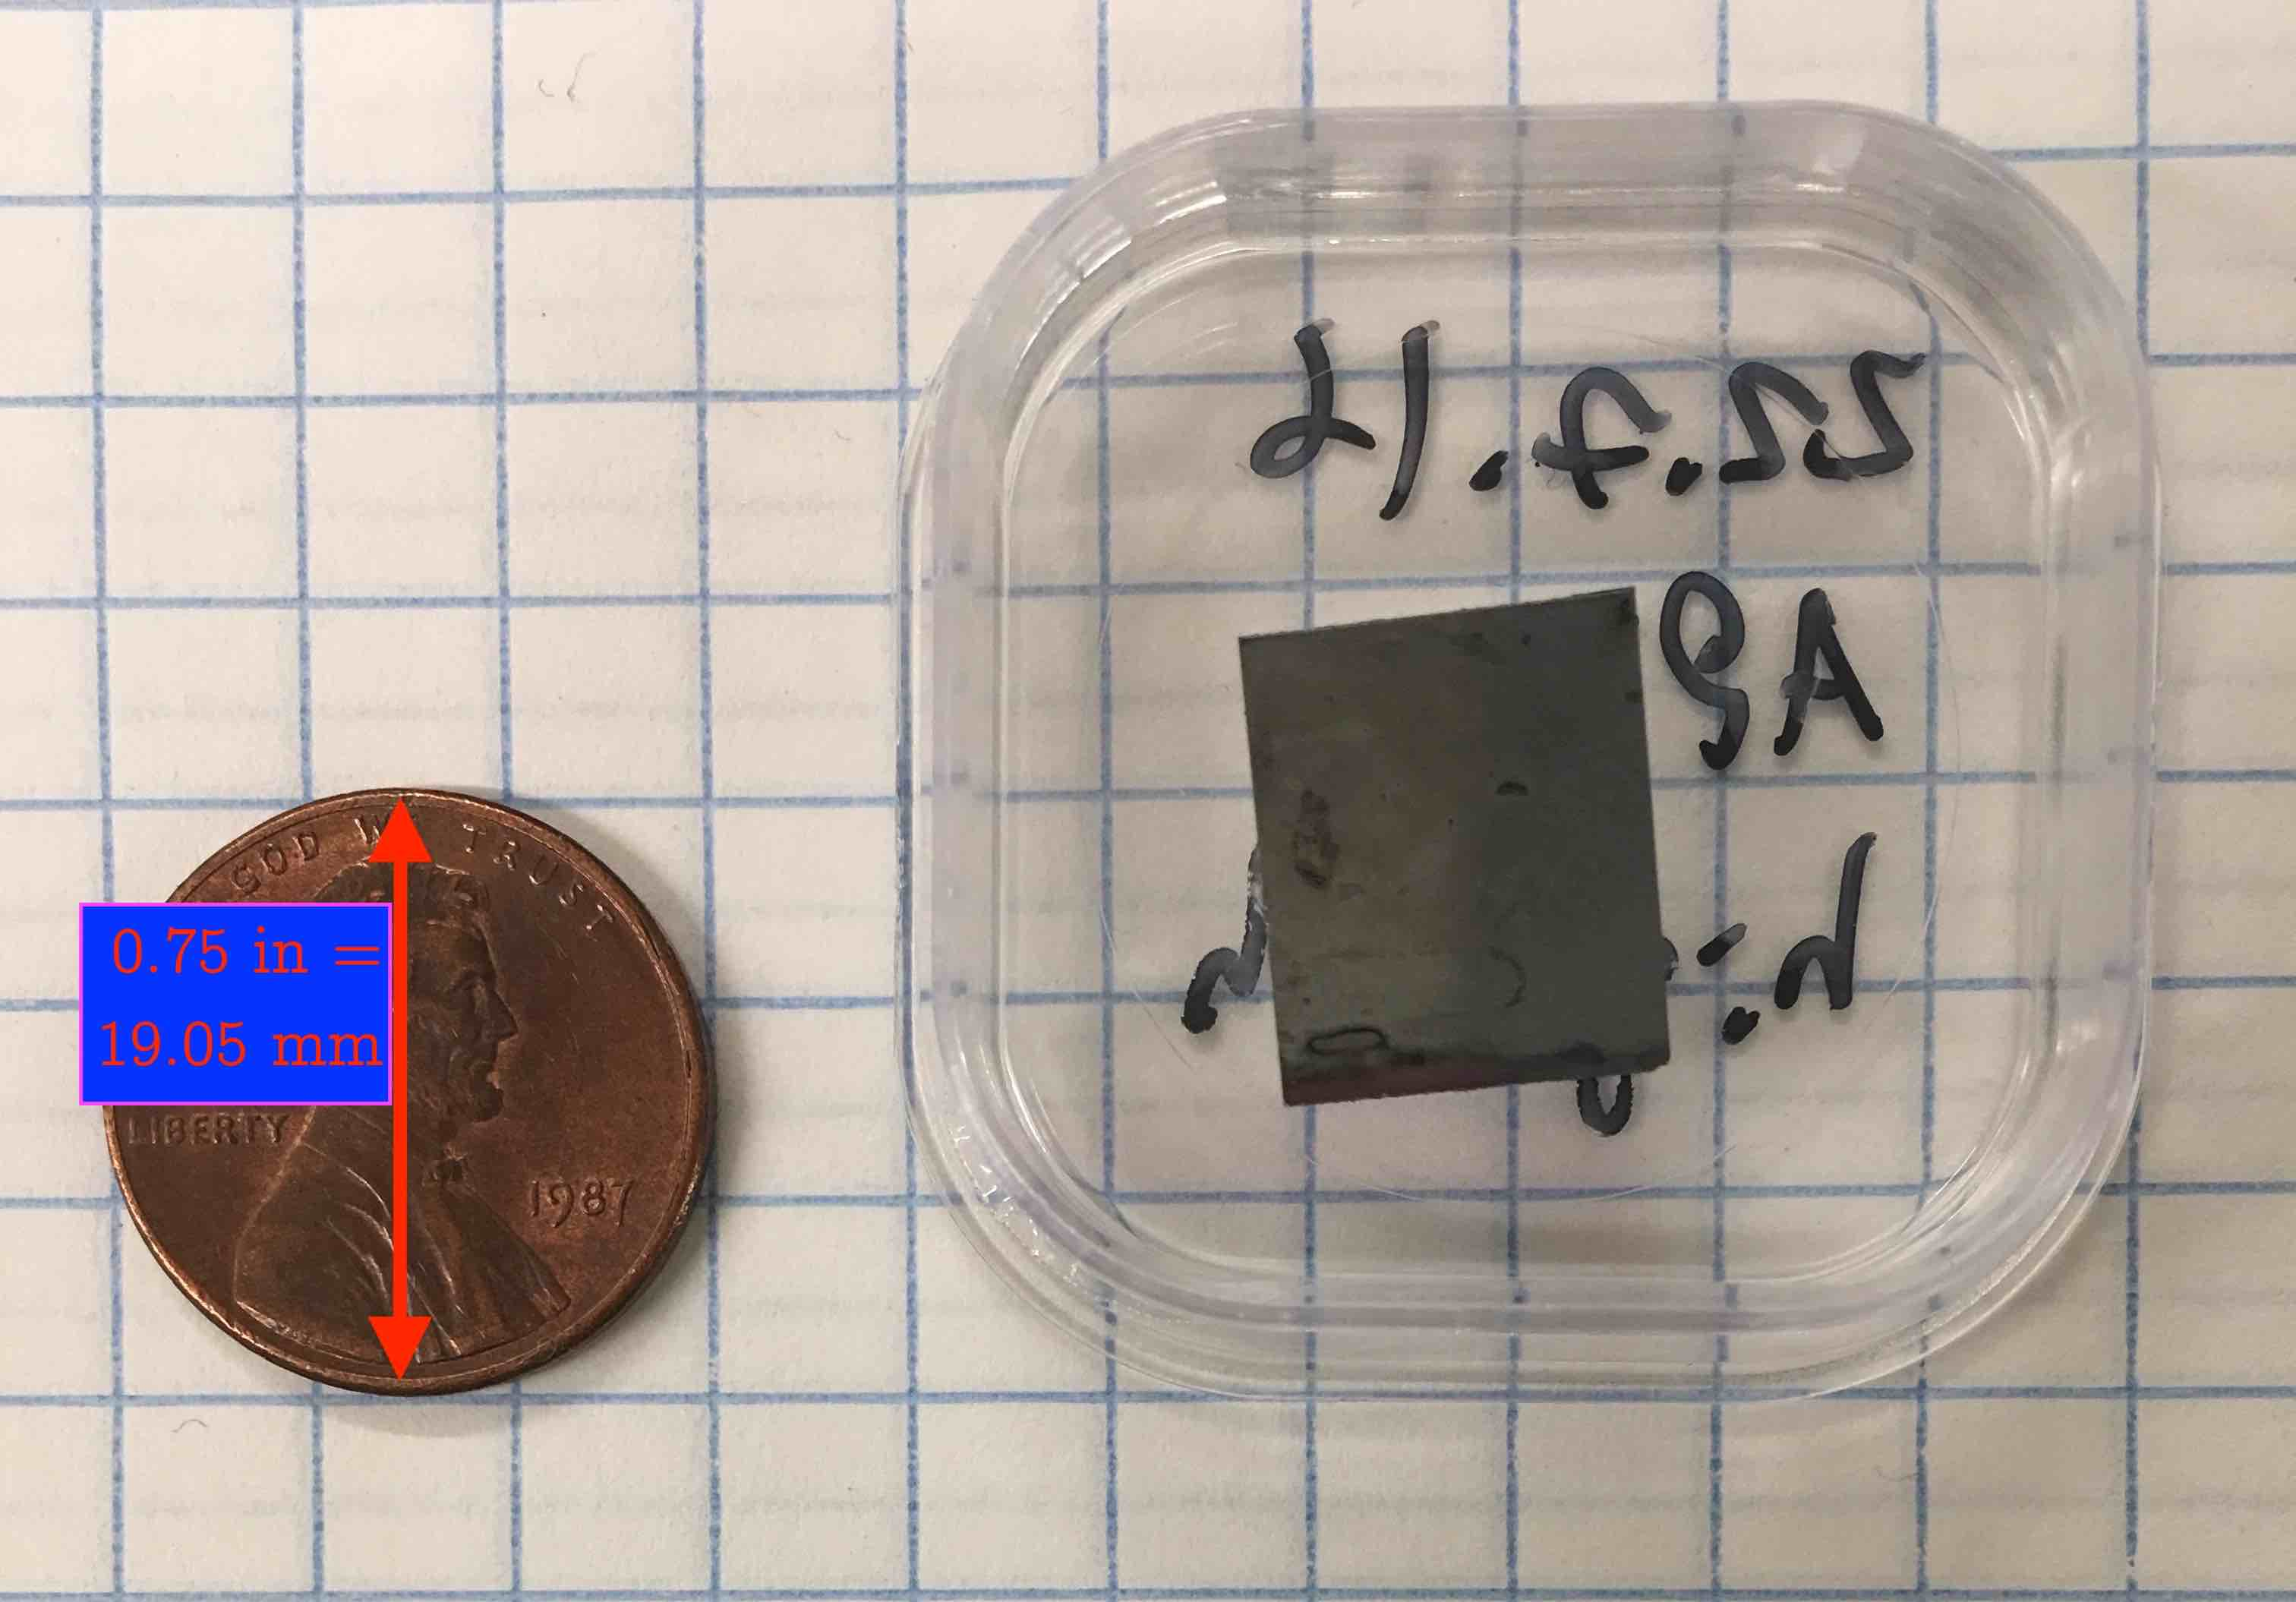
\includegraphics[width=3in]{./images/photo_of_thin_film_sample.jpg}%
}{%
  \caption{Top-down photo of the thin film sample of PbS(Th) analyzed in this work. US penny included for scale.\label{photo_of_thin_film_sample}}%
}
\capbtabbox{%
\begin{tabular}{|l|l|}\hline
Substrate						&	GaAs (100) \\\hline
Dimensions					&	1 cm x 1.5 cm \\\hline
Film thickness					&	$\sim$500 nm \\\hline
Grain size						&	$\sim$150 nm \\\hline
Th 228 concentration			&	0.15 ppm \\\hline
Total activity*					&	65 Bq \\\hline
Sample creation date			&	22 Jul 2016\\\hline
\end{tabular}
}{%
  \caption{Sample properties reported by Templeman et al. 2017 \cite{Templeman2017}. * Total activity measured a brief but unknown time after sample preparation. \label{sample_properties}}%
}
\end{floatrow}
\end{figure}


%[What about crystal misfit calculations? Can I just say that I neglected them, but that PbS and GaAs have pretty different lattice constants and it might actually matter.]

% \cite{patterson:risc,rad83}.  
% \cite{ellis:bulldog,pet87,coutant:precision-compilers}.  In these cases, the
% \cite{gib86}.
% These optimizations are described in detail in section~\ref{ch1:opts}.
% \section{Description of micro-optimization}\label{ch1:opts}
% \footnote{A description of the floating point format used is shown in figures~\ref{exponent-format}
% and~\ref{mantissa-format}.}.  
% A discussion of the mathematics behind unnormalized arithmetic is in appendix~\ref{unnorm-math}.

% \footnote{Using unnormalized numbers for math is not a new idea; a
% good example of it is the Control Data CDC 6600, designed by Seymour Cray.
% \cite{thornton:cdc6600} The CDC 6600 had all of its instructions performing
% unnormalized arithmetic, with a separate {\tt NORMALIZE} instruction.}.

% This is an example of how you would use tgrind to include an example
% of source code; it is commented out in this template since the code
% example file does not exist.  To use it, you need to remove the '%' on the
% beginning of the line, and insert your own information in the call.
%
%\tagrind[htbp]{code/pmn.s.tex}{Post Multiply Normalization}{opt:pmn}

% This is an example of how you would use tgrind to include an example
% of source code; it is commented out in this template since the code
% example file does not exist.  To use it, you need to remove the '%' on the
% beginning of the line, and insert your own information in the call.
%
%\tgrind[htbp]{code/be.s.tex}{Block Exponent}{opt:be}
